\documentclass[tikz, border=2pt]{standalone}
\begin{document}
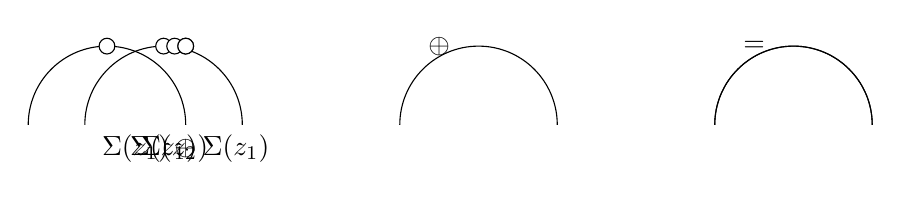
\begin{tikzpicture}[
    arc radius/.store in=\arcrad, arc radius=1cm,
    circle size/.store in=\csize, circle size=2mm,
    gap/.store in=\gap, gap=1cm,
    baseline=(current bounding box.center)
]

% Helper macro for a single arc with circle at apex and label below
\newcommand{\singlearc}[3]{% x, y, label
    \draw (#1,#2) arc[start angle=0, end angle=180, radius=\arcrad];
    \draw[fill=white] (#1-\arcrad,#2+\arcrad) circle[radius=\csize/2];
    \node at (#1-\arcrad,#2-0.3) {$#3$};
}

% Component 1: Σ(z₁)
\singlearc{0}{0}{\Sigma(z_1)}

% Component 2: ⊕
\node at (2.5,1) {$\oplus$};

% Component 3: Σ(z₂)
\singlearc{4}{0}{\Sigma(z_2)}

% Component 4: =
\node at (6.5,1) {$=$};

% Component 5: Result — Σ(z₁) ⊕ Σ(z₁)
% Top arc
\draw (8,0) arc[start angle=0, end angle=180, radius=\arcrad];
\draw[fill=white] (8-\arcrad,0+\arcrad) circle[radius=\csize/2];

% Bottom left arc
\draw (8-\arcrad,0) arc[start angle=0, end angle=180, radius=\arcrad];
\draw[fill=white] (8-2*\arcrad,0+\arcrad) circle[radius=\csize/2];

% Bottom right arc
\draw (8,0) arc[start angle=0, end angle=180, radius=\arcrad];
\draw[fill=white] (8-\arcrad,0+\arcrad) circle[radius=\csize/2];

% Label below result
\node at (8-\arcrad,-0.3) {$\Sigma(z_1) \oplus \Sigma(z_1)$};

\end{tikzpicture}
\end{document}